\documentclass[crop,tikz]{standalone}

\usetikzlibrary{
	positioning
}

\begin{document}

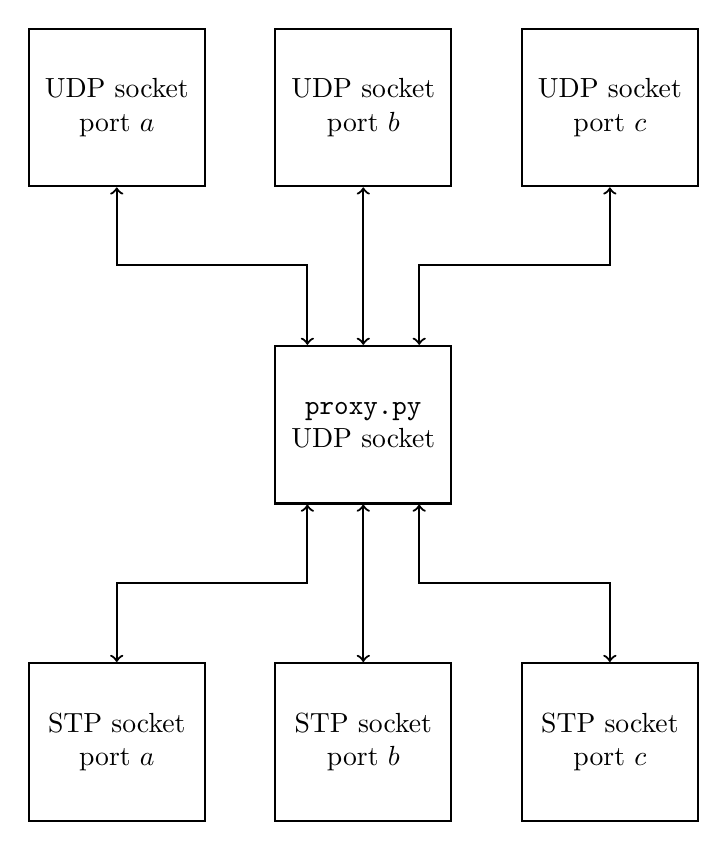
\begin{tikzpicture}[
	node distance =0mm,
	socket/.style = {
		rectangle,
		draw,
		thick,
		text width=2cm, align=center,
		minimum height=2cm
	},
]
	\node (listening) [socket, text width=2cm] {\texttt{proxy.py} UDP socket};
	
	\node (udp1) [socket, above left=2cm and 2cm of listening.north] {UDP socket port $a$};
	\node (udp2) [socket, above=2cm of listening.north] {UDP socket port $b$};
	\node (udp3) [socket, above right=2cm and 2cm of listening.north]{UDP socket port $c$};

	\draw[thick,<->] (udp1) |- node {} ++ (1,-2)  -|  (listening.125);
	\draw[thick,<->] (udp2) --  (listening.north);
	\draw[thick,<->] (udp3) |- node {} ++ (-1,-2)  -|  (listening.55);
	
	\node (stp1) [socket, below left=2cm and 2cm of listening.south] {STP socket port $a$};
	\node (stp2) [socket, below=2cm of listening.south] {STP socket port $b$};
	\node (stp3) [socket, below right=2cm and 2cm of listening.south] {STP socket port $c$};
	
	\draw[thick,<->] (listening.-125) |- node {} ++ (0,-1)  -|  (stp1);
	\draw[thick,<->] (listening.south) --  (stp2);
	\draw[thick,<->] (listening.-55) |- node {} ++ (0,-1)  -|  (stp3);
\end{tikzpicture}

\end{document}
